\documentclass[../main.tex]{subfiles}
\DoIfAndOnlyIfStandAlone{%
    \externaldocument{introduction}%
    \setcounter{chapter}{2}%
}%

\begin{document}

    \chapter{Linear Block Codes}

    \section{Hamming weight, Minimum Distance and Code Rate}

    The Hamming weight $w_H(x)$ of a codeword or vector $x$ is defined as the amount of non-zero elements or vector coordinates, which ranges from zero to length $n$ of said codeword.

    \begin{equation*}
        w_H(x) = \sum_{j=0}^{n-1} w_H(x_j), \text{ where } w_H(x_j) =
        \begin{cases}
            0, &\text{if } x_j = 0 \\
            1, &\text{if } x_j \neq 0
        \end{cases}
    \end{equation*}

    \noindent
    The Hamming distance $d_H(x,y)$ between two codewords or vectors $x$ and $y$ is defined as amount of elements or coordinates where $x$ and $y$ differ.

    \begin{equation*}
        d_H(x,y) = \sum_{j=0}^{n-1} w_H(x_j+y_j), \text{ where } w_H(x_j+y_j) =
        \begin{cases}
            0, \text{if } x_j=y_j \\
            1, \text{if } x_j \neq y_j
        \end{cases}
    \end{equation*}

    \begin{equation*}
        d_H(x,y) =  w_H(x,y)
    \end{equation*}

    \noindent
    The minimum distance $d_min$ of code $C$ is the minimum distance between two different codewords. The minimum distance for linear codes is equal to the minimum weight \autocite{bossert1999channel}. However, a codeword containing only zeros and therefore having a distance of zero is disregarded as the minimum distance cannot be zero.


    Let $x,y$ be codewords in code $C$. A received vector, which is the sent vector $x$ in $C$, plus error vector $e$ can only be corrected if the distance between any other codeword $y$ in $C$ fulfill

    \begin{equation*}
        d_{min}(x, x+e) < d_{min}(y, x+e) \text{ or } w_{min}(e) < w_{min}(x+y+e).
    \end{equation*}

    \noindent
    Therefore

    \begin{equation*}
         w_{min}(e) \leq \frac{d-1}{2},
    \end{equation*}

    \noindent
    where $d$ is the distance. This is written as

    \begin{equation*}
        t \leq \frac{d-1}{2} \text{ or } d \geq 2t+1,
    \end{equation*}

    \noindent
    where $t$ is the amount of errors that can be corrected.

    In general, a code $C$ of length $n$, with $M$ codewords, and a minimum distance $d=d(C)$, is called an $(n,M,d)$ code. Then M$ \leq q^{n-d+1}$ and the coderate of a $q$-ary $(n,M,d)$ code is at most $1-\frac{d-1}{n}$.

    A linear $q$-ary code of lenght $n$, with $k$ codewords or message symbols, and distance $d$ is called a $(n,k,d)$ code or $(n,k)$ code. The code rate is defined as

    \begin{equation*}
        R=\frac{log_qk}{n}.
    \end{equation*}

    \noindent
    If, according to Shannon's channel coding theorem, rate $R$ is less than capacity $C$, then the code exists but if rate $R$ is larger than capacity $C$, the error probability is 1 and the length of the codeword becomes infinite.


    \section{Singleton Bound}

    It is preferable to have a large minimum distance $d$ so that many errors can be corrected. Also, a large amount of codewords $M$ would allow for efficient use of bandwidth when transmitting over a noisy channel. Unfortunately, increasing $d$ tends to increase $n$ or decrease $M$. The Singleton bound is an upper bound for $M$ in terms of $n$ and $d$. A code that satisfies the Singleton bound is called a MDS code (maximum distance separable). The Singleton bound can be written as

    \begin{equation*}
        q^d \leq \frac{q^{n+1}}{M}
    \end{equation*}

    \noindent
    for the MDS code to obtain the largest possible value of $d$ for a given $n$ and $M$. Reed-Solomon codes are an important class of MDS codes \autocite{trappe2006introduction}.


    \section{Maximum-likelihood Decoding}

    There are two principles of decoding. In hard-decision decoding the received bits are believed to be either 1 or 0 in binary transmission. The decoding is done bit by bit. In soft-decision decoding, the received codewords may contain samples of bits with many values, not just 1 or 0. Calculating the closest error-free codeword is more complicated but soft-decision decoding has better performance than the hard-decision decoding.

    Assuming hard-decision decoding is used, the received codeword is decoded into its closest codeword measured by its smallest Hamming distance. This minimum probability of error principle is called Maximum-Likelihood or Minimum Distance Decoding \autocite{geisel1990tutorial}.

    The model of the binary symmetric channel (BSC) \autocite{mackay2003information} in \Cref{fig:binary_symmetric_channel} shows that the channel has binary input and output with an error probability, the channel is characterised by the following conditions if $c$ is the transmitted code and $r$ the received code:

    \begin{align*}
        \begin{rcases*}
            P(r=0|c=0) &= 1-p\\
            P(r=0|c=1) &= p\\
            P(r=1|c=0) &= p\\
            P(r=1|c=1) &= 1-p
        \end{rcases*} \text{ and } 0 \leq p \leq \frac{1}{2}\\
    \end{align*}

    Comparing all received codewords $r$ to all transmitted codewords $c$ as a direct way of correcting errors would not be inefficient. This means storing all $2k$ code vectors and performing equally as many comparisons for each received codeword, resulting in error vectors of which the vector with the smallest distance is probably the transmitted codeword. A more practical decoding method would be Syndrome decoding which will be described in \Cref{sec:syndrome_decoding}.


    \section{Hamming Codes}

    Hamming constructed a code where he added three additional bits to four information bits. These additional or parity bits are chosen based on the information bits in the following manner:

    \begin{align*}
        p_1 &= i_1 + i_2 + i_4\\
        p_2 &= i_1 + i_3 + i_4\\
        p_3 &= i_2 + i_3 + i_4
    \end{align*}

    \noindent
    and form the codeword $c=(i_1, i_2, i_3, i_4, p_1, p_2, p_3)$ . Hamming codes are block codes. This means that a fixed block of input data is processed into a fixed block of output data. A code is called a systematic code if the codeword starts with the information bits, followed by the parity bits, as shown in \Cref{fig:systematic_codeword}. A non-systematic code has the information bits in a different order. The parity bits are the result of a modulo 2 addition, so if there is an even amount of bits, it gives 0 and 1 when there is an odd amount. If a single error occurs, i.e., a bit is flipped or reversed, the codeword no longer satisfies the equations.

    \begin{figure}[htp]
        \centering
        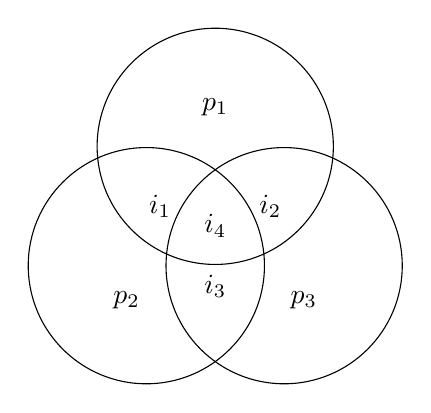
\begin{tikzpicture}[
                set/.style = {draw, circle, minimum size=3cm, align=center},
            ]
            \node (A) at (0,0) [set] {}; \node at (90:0.5cm) {$p_1$};
            \node (B) at (240:1.75cm) [set] {}; \node at (240:2.25cm) {$p_2$};
            \node (C) at (300:1.75cm) [set] {}; \node at (300:2.25cm) {$p_3$};

            \node at (barycentric cs:A=1,B=1) [left] {$i_1$};
            \node at (barycentric cs:A=1,C=1) [right] {$i_2$};
            \node at (barycentric cs:B=1,C=1) [below] {$i_3$};
            \node at (barycentric cs:A=1,B=1,C=1) [] {$i_4$};
        \end{tikzpicture}
        \caption{Relation between information and parity bits}
        \label{fig:information_and_parity_bits}
    \end{figure}

    \begin{figure}[htp]
        \centering
        \begin{tikzpicture}[
                box/.style = {draw, rectangle, minimum size=1cm, align=center},
            ]
            \node (data) [box, minimum width=6cm] {$k$ data bytes};
            \node (parity) [box, right=0cm of data] {$n-k$ parity bytes};
        \end{tikzpicture}
        \caption{An example of a systematic codeword of length $n$}
        \label{fig:systematic_codeword}
    \end{figure}

    \newpage

    \begin{figure}[htp]
        \centering
        \begin{tikzpicture}[
                            > = latex,
                   box/.style = {draw, minimum size=10mm},
                   add/.style = {draw, fill=gray!10, minimum size=10mm},
                   dot/.style = {circle, draw, fill, minimum size=1mm, inner sep=0mm, node contents={}},
            ]
            % data word nodes
            \node (di1) [box] at (0,0)  {$i_1$};
            \node (di2) [box] at (0,-1) {$i_2$};
            \node (di3) [box] at (0,-2) {$i_3$};
            \node (di4) [box] at (0,-3) {$i_4$};

            % code word nodes
            \node (ci1) [box] at (10,0)  {$i_1$};
            \node (ci2) [box] at (10,-1) {$i_2$};
            \node (ci3) [box] at (10,-2) {$i_3$};
            \node (ci4) [box] at (10,-3) {$i_4$};
            \node (cp1) [box] at (10,-4) {$p_1$};
            \node (cp2) [box] at (10,-5) {$p_2$};
            \node (cp3) [box] at (10,-6) {$p_3$};

            % mod 2 adder nodes
            \node (a1) [add] at (5,-4)   {$i_1+i_2+i_4$};
            \node (a2) [add] at (5,-5.5) {$i_1+i_3+i_4$};
            \node (a3) [add] at (5,-7)   {$i_2+i_3+i_4$};

            % connection nodes
            \node (n1) [dot, right=0.5cm of di1];
            \node (n2) [dot, right=1cm of di2];
            \node (n3) [dot, right=1.5cm of di3];
            \node (n4) [dot, right=2cm of di4];
            \node (n5) [left=1cm of cp2] {};
            \node (n6) [left=0.5cm of cp3] {};

            % connections
            \draw (di1) edge (n1); \draw[->] (n1) edge (ci1);
            \draw (di2) edge (n2); \draw[->] (n2) edge (ci2);
            \draw (di3) edge (n3); \draw[->] (n3) edge (ci3);
            \draw (di4) edge (n4); \draw[->] (n4) edge (ci4);
            % i1
            \draw[->] (n1) |- node[dot] {} (a1.south west);
            \draw[->] (n1) |- (a2.south west);
            % i2
            \draw[->] (n2) |- node[dot] {} (a1.west);
            \draw[->] (n2) |- (a3.south west);
            % i3
            \draw[->] (n3) |- node[dot] {} (a2.west);
            \draw[->] (n3) |- (a3.west);
            % i4
            \draw[->] (n4) |- node[dot] {} (a1.north west);
            \draw[->] (n4) |- node[dot] {} (a2.north west);
            \draw[->] (n4) |- (a3.north west);
            % p1
            \draw[->] (a1.east) -- (cp1.west);
            % p2
            \draw[->] (a2.east) -| (n5.center) (n5.center) |- (cp2.west);
            % p3
            \draw[->] (a3.east) -| (n6.center) (n6.center) |- (cp3.west);

            % legends
            \coordinate[above=0.25cm of di1, label={4-bit data word}];
            \coordinate[above=0.25cm of ci1, label={7-bit code word}];
            \coordinate[below=0.5cm of a3, label={modulo 2 adders}];
        \end{tikzpicture}
        \caption{ Hamming (7,4) encoder.}
        \label{fig:hamming_encoder}
    \end{figure}

    The decoder receives a seven-bit codeword $r=(i'_1, i'_2, i'_3, i'_4, p'_1, p'_2, p'_3)$. With an algebraic method known as syndrome decoding it is possible to determine the position of the error:

    \begin{align*}
        s_1 &= p'_1 + i'_1 + i'_2 + i'_4\\
        s_2 &= p'_2 + i'_1 + i'_3 + i'_4\\
        s_3 &= p'_3 + i'_2 + i'_3 + i'_4
    \end{align*}

    \noindent
    The three-bit syndrome $(s_1, s_2, s_3)$ returns $(0, 0, 0)$ when a received codeword contains no errors. There are seven more possible syndromes, each corresponding to the position of the error in the received codeword. The decoder then inverts the detected bit to counter the error.

    \newpage

    \begin{figure}[htp]
        \centering
        \begin{tikzpicture}[
                        > = latex,
                add/.style = {draw, fill=gray!10, minimum size=10mm, align=center},
                box/.style = {draw, minimum size=10mm, align=center},
                dot/.style = {circle, draw, fill, minimum size=1mm, inner sep=0mm, node contents={}},
                sum/.style = {circle, draw, minimum size=5mm,
                            path picture={\draw[thick,shorten <=1.5mm,shorten >=1.5mm,-]
                                            (\ppbb.north) edge (\ppbb.south)
                                            (\ppbb.west)  edge (\ppbb.east);
                                            },% end of path picture /node content/
                            node contents={}},
            ]
            % code word nodes
            \node (ci1) [box] at (0,0)  {$i'_1$};
            \node (ci2) [box] at (0,-1) {$i'_2$};
            \node (ci3) [box] at (0,-2) {$i'_3$};
            \node (ci4) [box] at (0,-3) {$i'_4$};
            \node (cp1) [box] at (0,-4) {$p'_1$};
            \node (cp2) [box] at (0,-5) {$p'_2$};
            \node (cp3) [box] at (0,-6) {$p'_3$};

            % data word nodes
            \node (di1) [box] at (10,0)  {$i_1$};
            \node (di2) [box] at (10,-1) {$i_2$};
            \node (di3) [box] at (10,-2) {$i_3$};
            \node (di4) [box] at (10,-3) {$i_4$};

            % mod 2 adder nodes
            \node (a1) [add, minimum height=1.5cm] at (5.5,-4.5)   {error at\\$i_1, i_2, i_4$\\or $p_1$};
            \node (a2) [add, minimum height=1.5cm] at (5.5,-6.5) {error at\\$i_1, i_3, i_4$\\or $p_2$};
            \node (a3) [add, minimum height=1.5cm] at (5.5,-8.5)   {error at\\$i_2, i_3, i_4$\\or $p_3$};

            % error correction nodes
            \node (e) [add, minimum height=5cm] at (8,-6.5) {error\\correction\\logic};
            \node (s1) [sum, left=0.5cm of di1];
            \node (s2) [sum, left=1cm of di2];
            \node (s3) [sum, left=1.5cm of di3];
            \node (s4) [sum, left=2cm of di4];

            % connection nodes
            \node (n1) [dot, right=2cm of ci1];
            \node (n2) [dot, right=2.5cm of ci2];
            \node (n3) [dot, right=3cm of ci3];
            \node (n4) [dot, right=3.5cm of ci4];
            \node (n5) [right=1.5cm of cp1] {};
            \node (n6) [right=1cm of cp2] {};
            \node (n7) [right=0.5cm of cp3] {};

            % connections
            \draw (ci1) edge (n1); \draw[->] (n1) edge (s1) (s1) edge (di1);
            \draw (ci2) edge (n2); \draw[->] (n2) edge (s2) (s2) edge (di2);
            \draw (ci3) edge (n3); \draw[->] (n3) edge (s3) (s3) edge (di3);
            \draw (ci4) edge (n4); \draw[->] (n4) edge (s4) (s4) edge (di4);
            % i'1
            \draw[->] (n1) |- node[dot] {} \findmid{0.667}{a1.south west}{a1.west};
            \draw[->] (n1) |- \findmid{0.667}{a2.south west}{a2.west};
            % i'2
            \draw[->] (n2) |- node[dot] {} \findmid{0.667}{a1.north west}{a1.west};
            \draw[->] (n2) |- \findmid{0.667}{a3.south west}{a3.west};
            % i'3
            \draw[->] (n3) |- node[dot] {} \findmid{0.667}{a2.north west}{a2.west};
            \draw[->] (n3) |- \findmid{0.667}{a3.north west}{a3.west};
            % i'4
            \draw[->] (n4) |- node[dot] {} (a1.north west);
            \draw[->] (n4) |- node[dot] {} (a2.north west);
            \draw[->] (n4) |- (a3.north west);
            % p'1
            \draw [->] (cp1.east) |- (n5.center) (n5.center) |- (a1.south west);
            % p'2
            \draw [->] (cp2.east) |- (n6.center) (n6.center) |- (a2.south west);
            % p'3
            \draw[->] (cp3.east) |- (n7.center) (n7.center) |- (a3.south west);
            % s1
            \draw[->] (a1.east) node[above right]{$s_1$} to (\tikztostart -| e.west);
            % s2
            \draw[->] (a2.east) node[above right]{$s_2$} to (\tikztostart -| e.west);
            % s3
            \draw[->] (a3.east) node[above right]{$s_3$} to (\tikztostart -| e.west);
            % e1
            \draw[<-] (s1.south) to (\tikztostart |- e.north);
            % e2
            \draw[<-] (s2.south) to (\tikztostart |- e.north);
            % e3
            \draw[<-] (s3.south) to (\tikztostart |- e.north);
            % e4
            \draw[<-] (s4.south) to (\tikztostart |- e.north);

            % legends
            \coordinate[above=0.25cm of di1, label={Decoded 4-bit data word}];
            \coordinate[above=0.25cm of ci1, label={Received 7-bit code word}];
            \coordinate[below=0.5cm of a3, label={modulo 2 adders}];
        \end{tikzpicture}
        \caption{ Hamming (7,4) decoder.}
        \label{fig:hamming_decoder}
    \end{figure}

    \autocite{bose2008information} considered the space of $q$-ary $m$-tuples, where every $q$-ary vector of length $m$ can be represented by its endpoint in this space. Hence, we can represent every codeword as a point in this space, and all codewords at a Hamming distance of $t$ or less would lie within the sphere centred at the codeword and with a radius of $t$.

    \begin{figure}[h!tp]
        \centering
        \begin{tikzpicture}[
                         > = latex,
             sphere/.style = {draw, circle, minimum size=3cm, align=center},
                dot/.style = {circle, draw, fill, minimum size=1mm, inner sep=0mm, node contents={}},
            ]
            % nodes
            \node (c1) at (0,0) [sphere] {}; \node at (c1.center) [dot] {}; \node [right=0.1cm of c1.center] {$c_1$};
            \node (c2) at (5,0) [sphere] {}; \node at (c2.center) [dot] {}; \node [right=0.1cm of c2.center] {$c_2$};
            \node (a) [below=1cm of c1] {};
            \node (b) [below=1cm of c2] {};

            % lines
            \draw[dotted] (a.center) -- (c1.center);
            \draw[dotted] (b.center) -- (c2.center);
            \draw[->] (c1.center) -- node[above right]{$t$} (c1.north west);
            \draw[->] (c2.center) -- node[above right]{$t$} (c2.north west);
            \draw[<->] (a.center) -- node[above]{$d > 2t + 1$} (b.center);

            \end{tikzpicture}
        \caption{Decoding sphere}
        \label{fig:decoding_sphere}
    \end{figure}


    \section{Syndrome Decoding} \label{sec:syndrome_decoding}

    \autocite{trappe2006introduction} define linear $(n,k)$ code of dimension $k$ and length $n$ over a field $F$ as a $k$-dimensional subspace of $F^n$. For example, a linear binary code, of length $n$ and dimension $k$ is a set of $2^k$ binary codewords or $n$-tuples, such that the sum of any two codewords is always a codeword. To construct such a linear $(n,k)$ code, we choose a $k \times n$ matrix known as generator matrix. The rows have to be linearly independent to produce unique codewords.

    Generator matrix $G$ is taken so that $G=[I_k,P]$, where $I_k$ is the $k \times k$ identity matrix which determine the codewords and $P$ is a $k \times (n-k)$ matrix that provides redundancy, the parity matrix. Now every codeword $c$ of code $C$ can be expressed as a linear combination of rows of $G$ by $c=i \cdot G$. We can now calculate the generator matrix for a systematic representation. For example, a systematic Hamming (7,4) code has the following generator matrix:

    \begin{equation*}
        G=[I_4|P]=
        \begin{bmatrix}
            1&0&0&0&1&1&0\\
            0&1&0&0&1&0&1\\
            0&0&1&0&0&1&1\\
            0&0&0&1&1&1&1
        \end{bmatrix}
    \end{equation*}

    \noindent
    The parity check matrix is then calculated as

    \begin{equation*}
        H=[-P^T|I_3]=
        \begin{bmatrix}
            1&1&0&1&1&0&0\\
            1&0&1&1&0&1&0\\
            0&1&1&1&0&0&1
        \end{bmatrix}
    \end{equation*}

    \noindent
    For example, encoding information bits $[1 1 0 0]$ gives

    \begin{equation*}
        \begin{bmatrix}
            1&1&0&0
        \end{bmatrix}
        \times
        \begin{bmatrix}
            1&0&0&0&1&1&0\\
            0&1&0&0&1&0&1\\
            0&0&1&0&0&1&1\\
            0&0&0&1&1&1&1
        \end{bmatrix}
        \equiv
        \begin{bmatrix}
            1&1&0&0&0&1&1
        \end{bmatrix}
    \end{equation*}

    \noindent
    Decoding received codeword $c'=[1100011]$ with syndrome decoding results in $[000]$ when no errors are detected. However, in our example an error was introduced in the fifth position of codeword $c'=[1100111]$, so we can expect a syndrome with non-zero elements.

    \begin{equation*}
        c' \times H^T =
        \begin{bmatrix}
            1&1&0&0&\underline{1}&1&1
        \end{bmatrix}
        \times
        \begin{bmatrix}
            1&1&0\\
            1&0&1\\
            0&1&1\\
            1&1&1\\
            \underline{1}&\underline{0}&\underline{0}\\
            0&1&0\\
            0&0&1
        \end{bmatrix}
        \equiv
        \begin{bmatrix}
            1&0&0
        \end{bmatrix}
    \end{equation*}

    \noindent
    The value $[100]$ can be looked up in parity check matrix $H$ and tells that the error occurred in the fifth position from the left. Correction based on syndrome requires more steps and asks for a matrix of all single error vectors. Codeword $c=[1100011]$ and received codeword $c=[1100111]$ give an error vector of $e=[0000100]$ or $c=c'+e$. Since we already know that $s=c' \cdot H^T$ and an error-free $c \cdot H^T$ has a syndrome with all zero elements, we now substitute $c'$ with $c+e$ because $c=c'+e$ is equivalent to $c'=c+e$ in binary.

    \begin{align*}
        s &= c' \cdot H^T\\
          &= (c+e) \cdot H^T\\
          &= c \cdot H^T + e \cdot H^T\\
          &= 0 + e \cdot H^T\\
          &= e \cdot H^T
    \end{align*}

    \noindent
    We can conclude that the syndrome solely depends on the error pattern and not on the transmitted codeword.


    \section{Cyclic Codes}

    Cyclic codes are widely used in data communication because their structure makes encoder and decoder circuitry simple. \autocite{hill1986first} defines code $C$ as cyclic $(n,k)$ code if $C$ is a linear code of length $n$ over a finite field and if any cyclic shift of a codeword is also a codeword. Thus,

    \begin{equation*}
        (c_0, c_1, c_2, \dots, c_{n-1}) \in  C \text{ and } (c_{n-1}, c_0, c_1, \dots, c_{n-2}) \in C.
    \end{equation*}

    Let $g(x)$ be the polynomial with the smallest degree. By dividing its highest coefficient, we may assume that the highest non-zero coefficient of $g(x)$ is 1. The polynomial $g(x)$ is called the generator polynomial for $C$, which must be a divisor of $x^n-1$ (in a binary field this is equal to $x^n+1$) with a degree of $n-k$. Subsequently, every cyclic code is a polynomial \autocite{trappe2006introduction}. The encoder for cyclic codes is then

    \begin{equation*}
        c(x)=i(x) \cdot g(x)
    \end{equation*}

    \noindent
    where $c(x)$ is the polynomial with degree $n-1$ of codeword $(c_0, c_1, c_2, \dots, c_{n-1})$ which is calculated as

    \begin{align*}
        c(x) &= \sum_{i=0}^{n-1} c_i \cdot x^i\\
             &= c_0 + c_1x + c_2x^2 + \dots +  c_{n-1}x^{n-1}
    \end{align*}

    \noindent
    and $i(x)$ is the information polynomial of degree $k-1$. Generator polynomial $g(x)$ must be of degree $n-k$.


    \section{BCH Codes}

    A BCH code is a cyclic polynomial code over a finite field with a particularly chosen generator polynomial. Hamming codes are the subset of BCH codes with $k=2^m-1-m$ and have an error correction of 1. Generally, a family of $t$-error correcting codes defined over finite fields $GF(q)$, where $2t+1<q$, are BCH codes or RS codes \autocite{hill1986first}. The main advantage of BCH codes is the ease with which they can be decoded using syndrome and many good decoding algorithms exist. A well-known decoding algorithm is the Berlekamp-Massey algorithm. This allows very simple electronic hardware to perform the task, making the need for a computer unnecessary. This implies that a decoding device may be small and consume little power. BCH codes allow control over block length and acceptable error thresholds, which makes them very flexible. This indicates that code can be designed to meet custom requirements. Another reason they are important is that there exist good decoding algorithms that correct multiple errors. Hocquenghem, as well as Bose and Ray-Chaudhuri, discovered the class of BCH codes, but not the decoding. Peterson developed the first decoding algorithm in 1960 followed by refinement from Berlekamp, Massey and many others \autocite{trappe2006introduction}.


    \subsection{Generating BCH Code}

    It is easy to generalise the construction of a $t$-error-correcting code of length $n=2^m-1$ over $GF(q)=\{0, 1, ..., q-1\}$ provided $2t+1 \leq n \leq q-1$. According to \autocite{hill1986first} it is not difficult to construct a binary BCH code over an extension field $GF(q^m)$. In order to obtain a cyclic code only the generator polynomial $g(x)$ is needed. For any integer $m \geq 3$ and $t < 2^{m-1}$, there exists a primitive BCH code with parameters:

    \begin{align*}
              n &= 2^m - 1\\
            n-k &\leq m \cdot t\\
        d_{min} &\leq 2t + 1
    \end{align*}

    Let $\alpha$ be a primitive $n$-th root of unity of $GF(2^m)$. For $1 \leq i \leq t$, let $m_{2i-1}(x)$ be the minimum polynomial of $\alpha_{2i-1}$. The degree of $m_{2i-1}(x)$ is $m$ or $a$ factor of $m$. The generator polynomial $g(x)$ of a $t$-error-correcting primitive BCH codes of length $2^m-1$ is given by

    \begin{equation*}
        g(x) = LCM \{m_1(x), m_2(x), m_3(x), ..., m_{2t-1}(x), m_{2t}(x)\}
    \end{equation*}

    \noindent
    with $LCM$ being Least Common Multiple, and because every even power of a primitive element has the same minimal polynomial as some odd power of the element, then $g(x)$ can be reduced to

    \begin{equation*}
        g(x) = LCM \{m_1(x), m_3(x), ..., m_{2t-1}(x)\}
    \end{equation*}

    \noindent
    The degree of $g(x)$ is $m \cdot t$ or less and so is the number of parity check bits, therefore $n-k \leq m \cdot t$ \autocite{lint1999introduction}.

    Generally a code is a BCH code over $GF (q )$ with $m , n , d , c \in N$ chosen such that q is a prime power and $2 \leq d \leq n$. Also, $m$ is the multiplicative order of $q$ modulo $n$ and $n$ is not divisible by $q$, so the greatest common divisor of $n$ and $q$ is 1 \autocite{lidl1998applied}. In special circumstances it is that,

    \begin{itemize}
        \item A BCH code with $c=1$ is called a narrow-sense BCH code;
        \item A BCH code with $n = q^m-1$ is called primitive;
        \item A narrow-sense BCH code with $n = q^m-1$ is called a Reed-Solomon code.
    \end{itemize}

    The consecutive roots of the generator polynomial may run from $\alpha^c, \dots, \alpha^{c+d-2}$ instead of $\alpha, \dots, \alpha^{d-1}$. As before, let $\alpha$ be a primitive $n$-th root of unity in $GF(q^m)$, and let $m_i(x)$ be the minimal polynomial over $GF(q)$ of $\alpha_i$ for all $i$. The generator polynomial of the BCH code is defined as the least common multiple $g(x) = LCM \{m_c(x), \cdots, m_{c+d-2}(x)\}$ \autocite{trappe2006introduction}.


    \subsection{Decoding BCH Code}

    BCH codes can be decoded in many way and it is most common that

    \begin{itemize}
        \item Syndromes values for are calculated for the received codeword;
        \item Error polynomials are calculated;
        \item Roots of these polynomials are calculated to obtain the location of errors;
        \item Error values are calculated at these locations.
    \end{itemize}

    Let code $C$ be a binary BCH code with distance $d \geq 3$. $C$ is a cyclic code of length $n$, with generating polynomial $g(x)$. There is a $n$-th root of unity $\alpha$ such that

    \begin{equation*}
        g(\alpha^{k+1}) = g(\alpha^{k+2}) = 0
    \end{equation*}

    \noindent
    for some integer $k$.

    \begin{equation*}
        \text{Let } H =
        \begin{bmatrix}
            1 & \alpha^{(k+1)} & \alpha^{2(k+1)} & \dots & \alpha^{(n-1)(k+1)}\\
            1 & \alpha^{(k+2)} & \alpha^{2(k+2)} & \dots & \alpha^{(n-1)(k+2)}
        \end{bmatrix}
    \end{equation*}

    \noindent
    If $c = (c_0, \dots, c_{n-1})$ is a codeword, then polynomial $m(x) = c_0 + c_1x + ... + c_{n-1}x^{n -1}$ is a multiple of $g(x)$, so

    \begin{equation*}
        m(\alpha^{k+1}) = m(\alpha^{k+2}) = 0
    \end{equation*}

    \noindent
    This may be rewritten in terms of $H$:

    \begin{equation*}
        c \cdot H^T = [c_0, \dots, c_{n-1}] \cdot
        \begin{bmatrix}
            1 & 1\\
            \alpha^{(k+1)} & \alpha^{(k+2)}\\
            \alpha^{2(k+1)} & \alpha^{2(k+2)}\\
            \vdots & \vdots\\
            \alpha^{(n-1)(k+1)} & \alpha^{(n-1)(k+2)}
        \end{bmatrix}
        = 0
    \end{equation*}

    \noindent
    $H$ is not necessarily a parity matrix for $C$, however, it can correct an error.

    Suppose codeword $c'=c+e$ is received with error vector $e=(e_0, ..., e_{n-1})$ . Assuming that there is one error, the algorithm for correcting one error is to write $c' \cdot H^T = (s_1, s_2)$.

    \begin{itemize}
        \item If $s_1 = 0$ then there is either no error or more than one error and we stop here.
        \item If $s_1 \neq 0$, take $\frac{s_2}{s_1}$ which results in a power $\alpha^{j-1}$ of $\alpha$.
    \end{itemize}

    The error is in position $j$ and $e_j=1$. Subtracting the error vector $e$ from the received codeword $c'$ gives the corrected codeword $c'_r$. For binary BCH codes it is only necessary to calculate the position, because the error value is always equal to 1. In non-binary BCH codes an additional error value polynomial is needed \autocite{trappe2006introduction}.


    \section{Reed-Solomon codes}

    RS codes, which are BCH codes, are used in applications such as spacecraft communications, compact disc players, disk drives, and two-dimensional bar codes. According to \autocite{bossert1999channel} the relationship between BCH and RS codes is such that RS codes comprise a subset of BCH codes and occasionally BCH codes comprise a subset of RS codes. \autocite{lint1999introduction} defines an RS code as a primitive BCH code of length $n=q-1$ over $GF(q)$.


    \subsection{Generating a Reed-Solomon code}

    Let $GF(q)$ be a finite field with $q$ elements and it generate a rather specific BCH code $C$ over $GF(q)$ of length $n$, called a Reed-Solomon code. Let $\alpha$ be a primitive $n$-th root of unity of $GF(q)$ and let code $C$ have a length of $n=q-1$. Now take $d$ so that $1 \leq d \leq n$ and the generator polynomial $g(x)$ is given by

    \begin{align*}
        g(x) &= \prod_{i=1}^{d-1} (x-\alpha^i)\\
             &= (x-\alpha)(x-\alpha^2)\dots(x-\alpha^{d-1})
    \end{align*}

    \noindent
    \autocite{trappe2006introduction} state that the minimum distance for $C$ is at least $d$. Since $g(x)$ is a polynomial of degree $d-1$, it has at most $d$ non-zero coefficients. Therefore, the codeword corresponding to the coefficients of $g(x)$ has a weight of at most $d$. It follows that $C$ has a weight of exactly $d$ and the dimension of $C$ is $n$ minus the degree of $g(x)$

    \begin{align*}
        n-deg(g) &= n-(d-1)\\
                 &= n+1-d
    \end{align*}

    \noindent
    Therefore, a Reed-Solomon code is a cyclic $(n, n+1-d, d)$ code with codewords corresponding to polynomials, where each $f(x)$ is a polynomial with coefficients in $GF(q)$ that cannot be factored into lower degree polynomials while assuming that the highest non-zero coefficient is 1:

    \begin{equation*}
        g(x) \cdot f(x) \text{ with } deg(f) \leq n-d
    \end{equation*}

    It follows that there are $q$ choices for each $n-d+1$ coefficients of $f(x)$, and thus there are $q$ $n-d+1$ codewords in code $C$. Therefore, an RS code is a MDS code since it makes the Singleton bound an equality.
\end{document}
